% =====================================================================
% preview_discovery_recall_mix_a -- R/ggplot2 -> tikzDevice (Frame-A, ESWA target)
% Canonical-JSON-only. Regenerate: Rscript submissions/frame-a-eswa/figures-r/make_figures_frame_a.R
% Provenance (JSON path :: field = plotted value), one line per series:
% SOURCE: results/frame_a/frame_a_verdict.json :: per_mix.MIX_A.discovery.recall_ci = [1.000, 1.000]
% SOURCE: results/frame_a/frame_a_verdict.json :: per_mix.MIX_A.discovery.n_damaging_gt = 35.0000
% =====================================================================
% WARNING: QA-PREVIEW-NOT-FOR-SUBMISSION (generated 2026-07-23 08:37:28 EDT)
% This file is NOT camera-ready. The MIX_A preview under figures-qa/
% !TEX encoding = UTF-8 Unicode
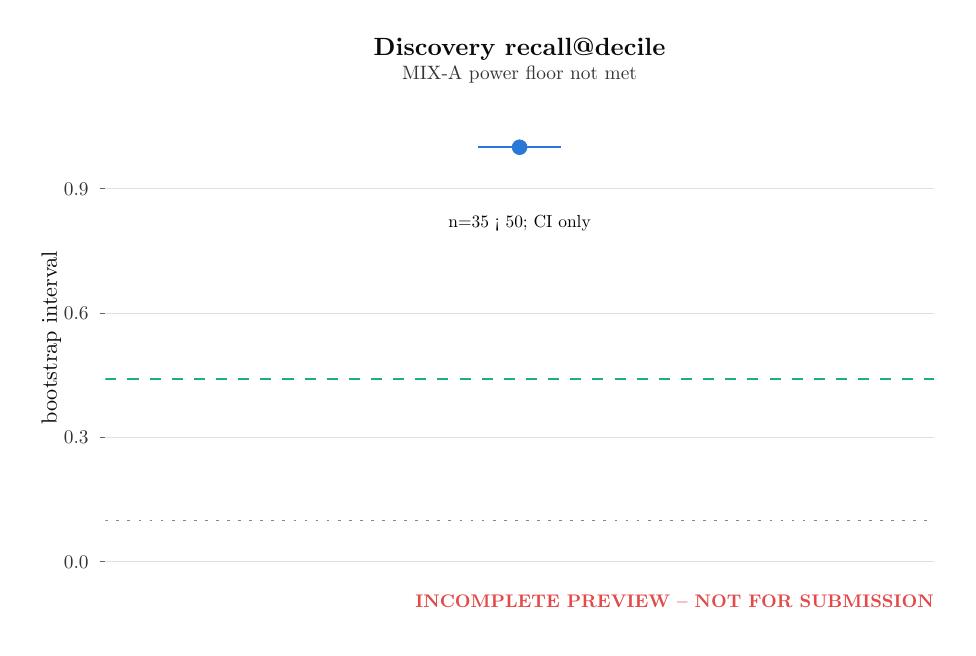
\begin{tikzpicture}[x=1pt,y=1pt]
\definecolor{fillColor}{RGB}{255,255,255}
\path[use as bounding box,fill=fillColor,fill opacity=0.00] (0,0) rectangle (332.44,216.81);
\begin{scope}
\path[clip] (  0.00,  0.00) rectangle (332.44,216.81);
\definecolor{fillColor}{RGB}{255,255,255}

\path[fill=fillColor] (  0.00,  0.00) rectangle (332.44,216.81);
\end{scope}
\begin{scope}
\path[clip] ( 28.06, 15.84) rectangle (327.44,193.67);
\definecolor{drawColor}{RGB}{225,224,217}

\path[draw=drawColor,line width= 0.3pt,line join=round] ( 28.06, 23.92) --
	(327.44, 23.92);

\path[draw=drawColor,line width= 0.3pt,line join=round] ( 28.06, 68.83) --
	(327.44, 68.83);

\path[draw=drawColor,line width= 0.3pt,line join=round] ( 28.06,113.73) --
	(327.44,113.73);

\path[draw=drawColor,line width= 0.3pt,line join=round] ( 28.06,158.64) --
	(327.44,158.64);
\definecolor{drawColor}{RGB}{137,135,129}

\path[draw=drawColor,line width= 0.5pt,dash pattern=on 1pt off 3pt ,line join=round] ( 28.06, 38.79) -- (327.44, 38.79);
\definecolor{drawColor}{RGB}{27,175,122}

\path[draw=drawColor,line width= 0.5pt,dash pattern=on 4pt off 4pt ,line join=round] ( 28.06, 89.89) -- (327.44, 89.89);
\definecolor{drawColor}{RGB}{42,120,214}

\path[draw=drawColor,line width= 0.8pt,line join=round] (162.78,173.61) --
	(192.72,173.61);

\path[draw=drawColor,line width= 0.8pt,line join=round] (177.75,173.61) --
	(177.75,173.61);

\path[draw=drawColor,line width= 0.8pt,line join=round] (162.78,173.61) --
	(192.72,173.61);
\definecolor{fillColor}{RGB}{42,120,214}

\path[draw=drawColor,line width= 0.3pt,line join=round,line cap=round,fill=fillColor] (177.75,173.61) circle (  2.65);
\definecolor{drawColor}{RGB}{0,0,0}

\node[text=drawColor,anchor=base,inner sep=0pt, outer sep=0pt, scale=  0.63] at (177.75,144.51) {n=35 < 50; CI only};
\end{scope}
\begin{scope}
\path[clip] (  0.00,  0.00) rectangle (332.44,216.81);
\definecolor{drawColor}{gray}{0.20}

\node[text=drawColor,anchor=base east,inner sep=0pt, outer sep=0pt, scale=  0.70] at ( 22.01, 21.51) {0.0};

\node[text=drawColor,anchor=base east,inner sep=0pt, outer sep=0pt, scale=  0.70] at ( 22.01, 66.42) {0.3};

\node[text=drawColor,anchor=base east,inner sep=0pt, outer sep=0pt, scale=  0.70] at ( 22.01,111.32) {0.6};

\node[text=drawColor,anchor=base east,inner sep=0pt, outer sep=0pt, scale=  0.70] at ( 22.01,156.23) {0.9};
\end{scope}
\begin{scope}
\path[clip] (  0.00,  0.00) rectangle (332.44,216.81);
\definecolor{drawColor}{gray}{0.40}

\path[draw=drawColor,line width= 0.3pt,line join=round] ( 26.06, 23.92) --
	( 28.06, 23.92);

\path[draw=drawColor,line width= 0.3pt,line join=round] ( 26.06, 68.83) --
	( 28.06, 68.83);

\path[draw=drawColor,line width= 0.3pt,line join=round] ( 26.06,113.73) --
	( 28.06,113.73);

\path[draw=drawColor,line width= 0.3pt,line join=round] ( 26.06,158.64) --
	( 28.06,158.64);
\end{scope}
\begin{scope}
\path[clip] (  0.00,  0.00) rectangle (332.44,216.81);
\definecolor{drawColor}{RGB}{11,11,11}

\node[text=drawColor,rotate= 90.00,anchor=base,inner sep=0pt, outer sep=0pt, scale=  0.80] at ( 10.51,104.75) {bootstrap interval};
\end{scope}
\begin{scope}
\path[clip] (  0.00,  0.00) rectangle (332.44,216.81);
\definecolor{drawColor}{gray}{0.20}

\node[text=drawColor,anchor=base,inner sep=0pt, outer sep=0pt, scale=  0.70] at (177.75,198.03) {MIX-A power floor not met};
\end{scope}
\begin{scope}
\path[clip] (  0.00,  0.00) rectangle (332.44,216.81);
\definecolor{drawColor}{RGB}{11,11,11}

\node[text=drawColor,anchor=base,inner sep=0pt, outer sep=0pt, scale=  0.90] at (177.75,206.60) {\bfseries Discovery recall@decile};
\end{scope}
\begin{scope}
\path[clip] (  0.00,  0.00) rectangle (332.44,216.81);
\definecolor{drawColor}{RGB}{227,73,72}

\node[text=drawColor,anchor=base east,inner sep=0pt, outer sep=0pt, scale=  0.66] at (327.44,  7.28) {\bfseries INCOMPLETE PREVIEW -- NOT FOR SUBMISSION};
\end{scope}
\end{tikzpicture}
